\chapter{Depth-of-Field}
As discussed in chapter \ref{ch:background} virtual cameras are able to take perfect color samples from every angle and thus create an image with infinite \gls{dof}.
However without expensive operations, like the simulation of a lens with path tracing, a virtual camera is only able to create perfect images.
As such the difficulty in simulating depth of field in real-time lies in combining images with infinite \gls{dof} into good approximation of real camera images.
The ideal method would be able to satisfy the following criteria:
\begin{itemize}
    \item Specification of a point-spread-function
    \item Per-pixel blur level control
    \item Lack of intensity leakage
    \item Lack of depth discontinuity artefacts
    \item Simulation of partial occlusion
    \item High performance
\end{itemize}

\todo{Explain intensity leakage, discontinuity artefacts and partial occlusion}

\section{Accumulation buffers}
The earliest method to generate a depth-of-field effect using traditional rasterization hardware was presented by Haeberli and Akeley. \cite{Haeberli.1990}
Their method introduces the use of an accumulation buffer to the rendering pipeline to simulate multiple effects, including motion blur and \gls{dof}.
The accumulation buffer is a region of memory used by the rendering hardware to accumulate and average the results of multiple rendering passes.
To simulate a depth-of-field effect the following steps are iterated:
\begin{enumerate}
    \item \textbf{Jittering:} The camera position is slightly disturbed. Commonly done by offsetting the principal point of the camera, but keeping the camera pointed at the same point in the scene
    \item \textbf{Rendering:} An image is created using the traditional rasterization pipeline
    \item \textbf{Accumulation:} The rendered image is added to the accumulation buffer.
\end{enumerate}
The jittering of the camera simulates the size of the individual image pixel of a real image sensor.
The images are then averaged to approximate the integration of all light paths hitting a sensor pixel.
As such out of focus objects will have varying positions in the rendered images and thus are spread out over their \gls{coc} in the final image.
This method therefore converges on the correct solution and does not suffer from the image artefacts mentioned earlier.

\begin{wrapfigure}{R}{0.4\linewidth}
\begin{center}
    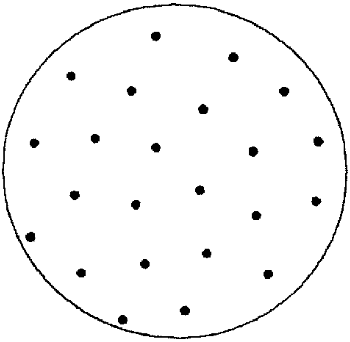
\includegraphics[width=0.4\textwidth]{images/sample-locations.png}
\end{center}
\caption{Position of sample location used to sample the aperture of the camera lens. \cite{Haeberli.1990}}
\label{fig:sample-pos}
\end{wrapfigure}

The specific approach to jittering the camera is subject to the individual implementation, but should move the camera parallel to the image plane.
Sampling points in a circular area may be used to simulate a circular aperture, but a hexagonal or octagonal sampling shape may be preferred for mechanical apertures.
Similarly the distribution of points may be adjusted achieve a specific \gls{psf}.
As such this approach great artistic flexibility.

To hide the individual frames a minimum density of samples must be taken to sufficiently cover the biggest \gls{coc} present in the image.
As such the amount of work needed to get acceptable results scales linearly with the \textbf{area} of the biggest \gls{coc} created by the scene.
Acceptable results are typically achieved with a single pass per 4 pixel area of the \gls{coc}.
This still results in 50 passes at a \gls{coc} with a 8 pixel radius. \cite{Demers.2005}
Thanks to the use of a traditional rasterization pipeline this method is often faster than ray-traced approaches.
However the high increase in the rendering workload excludes its use in all but the most CPU-bound real-time rendering workloads or as reference images.

\section{Single-Layer approaches}
To improve on the performance of accumulation buffers, several techniques have been developed, that limit themselves to a single rendering pass.
In addition to the color information in the frame buffer, all these techniques store the depth of each pixel in a separate z-buffer.
The main way the following methods differ is in their use of the given data to create the final image.
Due to the limitation on the information provided, all of the following methods exhibit some artifacts, that are accepted for the higher performance they offer.

The single-layer approaches can be categorized into two sub-categories based on the direction of how the final color for each pixel is calculated.

\subsection{Scattering methods}
The first method to generate depth of field, commonly referred to as \textit{splatting}, or \textit{forward-mapped z-buffer \gls{dof}} was introduced by Potmesil et al.\cite{Potmesil.1981}
It uses the fact that the image of pinhole camera stores the light intensity for \textbf{most} directions that hit the sensor.
With the additional information of the depth we can calculate the \gls{coc} of each light ray.
To efficiently calculate the final color of a pixel, a sprite with the calculated \gls{coc} size is placed at its position.
The color of the sprite is taken from the original pixel while its alpha value is inversely proportional to the size of the \gls{coc}.
As with the use of accumulation buffers the shape an color of the sprite can be modified to simulate a specific \gls{psf}.
The sprite is then placed at the original distance and second rendering pass is used to generate the final image.

The resulting image is a very close approximation of an image generated by the accumulation buffer method.
The main visual imperfection created by this method is the lack of partial occlusion.
This is barely noticeable in static scenes, but causes bright objects to suddenly appear when coming into view behind other objects.
As this method relies on the interaction of transparent sprites, we must each sprite for accurate transparency.
This log-linear time complexity in regard to the resolution is the main drawback of this method.
While real-time application such as video games may not find this performance acceptable, the high quality make it an attractive option for providing previews of renders.\cite{Demers.2005}
Real-time performance can be achieved when using commutative blending.

Lee et al. \cite{Lee.2008} present a modified version of this algorithm that splits the scene into three layers.
Splatting is done via commutative blending onto three separate layers.
A second rendering pass of hidden scene elements is done to alleviate the partial occlusion problems of the traditional method.

\subsection{Gathering methods}
The second single-layer method was introduced by Rokita et al. \cite{Rokita.1993} and gathers the color information for each pixel of the final image by consulting the image of a pinhole camera.
It is also commonly referred to as \textit{reverse-mapped z-buffer \gls{dof}}.\cite{Gilham.2007}

The simplest implementation of this approach is achieved by generating a mip-map of the rendered screen texture.
Then the \gls{coc} is calculated for each pixel and is used to perform trilinear interpolation to find the final color value.
To access the depth buffer was an issue in early graphics APIs and early GPUs and had to be manually created.
However since the introduction of OpenGL 2.0 and DirectX 9 and their compatible hardware, access to depth buffer information is widely supported.
As this process is easily parallelized per pixel and has hardware support on modern GPUs, it is very performant on modern graphics hardware.
However the simple implementation generates multiple objectionable visual artefacts, that make the simple implementation unsuitable for most applications.\cite{Demers.2005, Hammon.2008}

The worst artifact is caused by the single depth lookup per pixel.
In the case of a real camera system, objects and by extension their outline are blurred.
A point at the edge of an out of focus object will spread out over the focused background.
This causes a smooth transition from blurry objects in the foreground to the focused objects.
Taking a single depth look up per pixel will only blur the image section of the object and not the entire object.
As such a hard boundary between the foreground and the focused part of the image will appear in the final image.
This artifact can be seen in figure \ref{fig:depth-discontinuity}.\cite{Demers.2005}

%\begin{wrapfigure}{R}{0.5\linewidth}
%\begin{center}
%    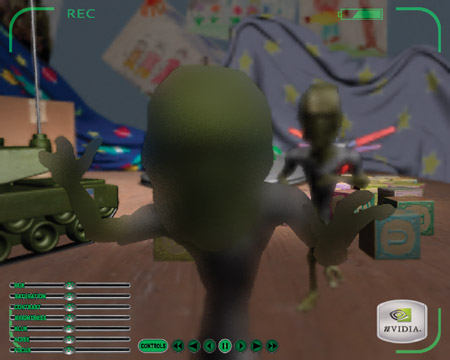
\includegraphics[width=0.48\textwidth]{images/depth-discontinuity.jpg}
%\end{center}
%\caption{Depth Discontinuity causes hard edges around blurred objects. \cite{Demers.2005}}
%\label{fig:depth-discontinuity}
%\end{wrapfigure}

\begin{figure}[h]
    \centering
    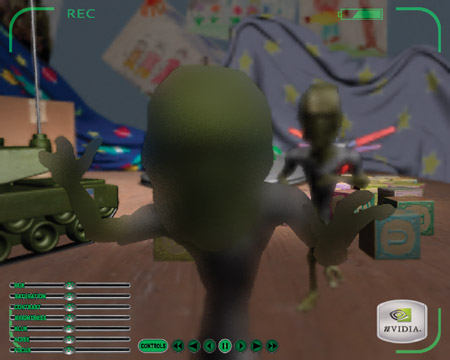
\includegraphics[width=0.5\textwidth]{images/depth-discontinuity.jpg}
    \caption{Depth discontinuity causes hard edges around blurred objects. \cite{Demers.2005}}
    \label{fig:depth-discontinuity}
\end{figure}

Hammond \cite{Hammon.2008} presents an approach to resolve this issue and generate a more natural \gls{dof} for foreground objects.
A full-screen pass that calculates the \gls{coc} for each foreground object is calculated and stored as a texture.
To calculate the \gls{coc} equation \ref{eq:coc-expanded} may be used, but other options are available for more artistic control.
Especially in first-person games it is often desirable for the player's weapons or other important objects to always remain in focus.
To achieve this Hammond Jr. proposes using negative depth values to indicate pixel containing to the view model.
Pixel in focus or background are assigned a \gls{coc} of zero.
This texture is first downsampled to one-fourth resolution along both axis for better performance.
The downsampled texture is then blurred using a Gaussian blur to eliminate edges between foreground and focused and background objects.
The final \gls{coc} value used by this method is given by:
\begin{align}
    D = 2 \cdot max(D_0, D_B) - D_0.
\end{align}
Where $D_0$ represents the downsampled depth-texture and $D_B$ represents the blurred depth-texture for each pixel.
A final full-screen pass is finally done to apply a variable width blur by interpolating between the original pinhole image and downsampled versions of it.
Lee et al. \cite{Lee.2009} improves on Hammond's method by using non-linear interpolation during the blurring step.
However both methods still suffer from the fundamental limitations of this approach.
As such they both blur object behind transparent foreground objects and struggle with high blur radii.

Another artefact created by simple trilinear filtering are bilinear interpolation artefacts of the magnified layers.
These causes a stair-stepped pattern to appear in blurred objects and can be seen in figure \ref{fig:trilinear-filtering}.
To alleviate these artifacts a different downsampling method may be used.
Another option is to apply a Gaussian blur to the downsampled images to simulate a more realistic blur.
Different kernels may be chosen to simulate a particular \gls{psf}.
However for optimal performance a separable kernel should be used.\cite{Demers.2005, Gilham.2007}

%\begin{wrapfigure}{R}{0.5\linewidth}
%\begin{center}
%    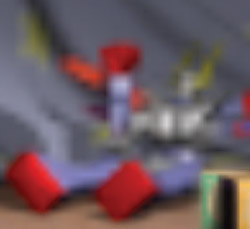
\includegraphics[width=0.48\textwidth]{images/trilinear-filtering.jpg}
%\end{center}
%\caption{Magnification Artifacts with Trilinear Filtering \cite{Demers.2005}}
%\label{fig:trilinear-filtering}
%\end{wrapfigure}

\begin{figure}[h]
    \centering
    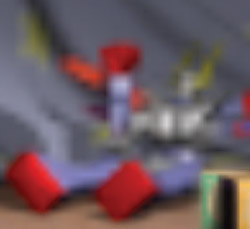
\includegraphics[width=0.5\textwidth]{images/trilinear-filtering.jpg}
    \caption{Magnification artifacts with Trilinear Filtering \cite{Demers.2005}}
    \label{fig:trilinear-filtering}
\end{figure}

The final artefact created by this approach is also caused at the border between foreground and in focus objects.
As the image of blurred objects is blurred indiscriminately, the blurring process will also use color information of in focus areas.
As such focused image areas will spread into blurred areas, as seen in figure \ref{fig:pxl-bleeeding}.
This artefact is called \textit{intensity-} or \textit{pixel-bleeding}.\cite{Demers.2005}
One approach to reduce these artefacts proposed by Lee et al. \cite{Lee.2009} is the use of an \textit{anisotropic mipmapping} scheme to preclude the effects of adjacent pixel.

\begin{figure}[h]
    \centering
    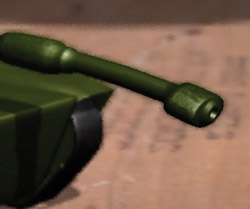
\includegraphics[width=0.5\textwidth]{images/pixel-bleeding.jpg}
    \caption{Pixel-bleeding artefacts of focused tank \cite{Demers.2005}}
    \label{fig:pxl-bleeeding}
\end{figure}

\section{Multi-Layer approaches}
Multi-layer approaches have been developed to address the problem of intensity leakage and the lack of partial occlusion of single-layer approaches.
In multi-layer approaches the rendered pin-hole image is first decomposed into several sub-images each representing a layer in the scene.
The layers are then separately blurred and recombined at the end.
How the image is separated and how the sub-images are combined are the main points of difference between different methods.
In the following we will present a method presented by Kraus and Strengert \cite{Kraus.2007}, which builds upon a method presented by Barsky et al.\cite{BrianA.Barsky.2005}

First a normal pinhole image with according depth information is rendered and stored as textures.
This image is then split into multiple sub-images denoted by $I^{(i)}$.
Each layer is initialized to the input pinhole image and its depth map.
For each layer a value $z^{(i)}$ is defined by:
\begin{align}
    z^0 &= z_{focal} \\
    z^i &= \frac{z_{focal}}{1 - r^{(i)}_{pix} / r^{(z \rightarrow \infty)}_{pix}}
\end{align}
Where by $r^{(i)}_{pix}$ represents the blur radius given by the blur method for each layer.
Negative values of $i < 0$ represent the foreground, conversely $i > 0$ represent the background.
Due to a following step, all pixel with depth values of $z < z^{(i+2)}$ for layer $I^{(i)}$ are discarded and set to transparent black.\cite{Kraus.2007}

In the next step the discarded foreground pixel of each layers are disoccluded.
This step is mostly done to alleviate the problem of intensity leakage.
A method of GPU-based pyramidal interpolation presented by Strengert et al. \cite{Strengert.2006} is used to interpolate color and depth information across discarded pixel.
To generate information for the missing pixel, first the available pixel and their alpha values are averaged onto a texture with half resolution in both dimensions, similar to the generation of mip-maps.
Is the synthesis step of this method, each layer is searched for pixel with missing color information (i.e. with alpha value of 0), is given the color of the layer directly above.
This is repeated until the bottom layer is reached, where all RGB-components are divided by their alpha value to get their final color.
This offers up new color information for the blurring step and prevents the pixel-bleeding artefacts of caused by closer layers as seen in figure \ref{fig:pxl-bleeeding}.

\begin{figure}[h]
    \centering
    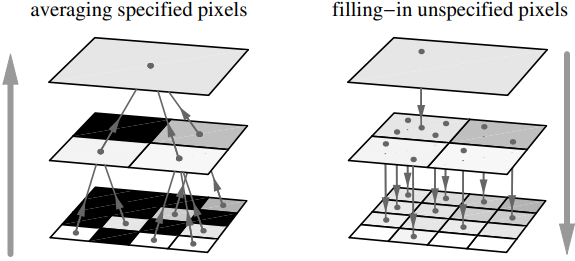
\includegraphics[width=0.5\textwidth]{images/pyramidal-interpolation.png}
    \caption{Pyramidal Interpolation of missing pixel.\cite{Kraus.2007}}
    \label{fig:pyramidal-interpolation}
\end{figure}

The main difficulty of multi-layer approaches lies in hiding the boarders between individual layers.
To address this issue, this method "matts" each layer $I^{(i)}$ using a piecewise linear function $\omega^{(i)}(z)$ seen in figure \ref{fig:matt-func}.
Each color component is multiplied by $\omega^{(i)}(z)$.
Thus $\omega^{(i)}(z)$ can be viewed as a weighting function between layers and contributes to a smooth transition between layers in the final blending.
This step must be done before the blurring of individual layers to ensure the blurring step does not use color information of layers further back.\cite{Kraus.2007}

\begin{wrapfigure}{R}{0.5\linewidth}
\begin{center}
    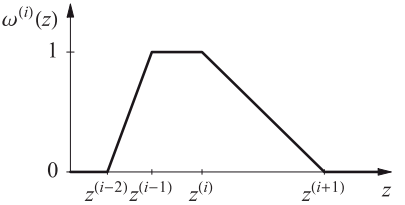
\includegraphics[width=0.48\textwidth]{images/matt-function.png}
\end{center}
\caption{The matting function $\omega^{(i)}(z)$ for sub-image $I^{(i)}$.\cite{Kraus.2007}}
\label{fig:matt-func}
\end{wrapfigure}

In this implementation of the method the blurring of the sub-images is again done via the pyramidal method introduced by Strengert et al. \cite{Strengert.2006}.
To generate a blur of width $2^l$ the original image is copied in to level $G_0$ of the pyramid and levels $G_1$ to $G_l$ are computed.
The synthesis of the final blurred sub-image is done as discussed above.
Kraus et al. propose the use of a scaled blur radius of
\begin{align}
    r^{(0)}_{pix} &= 0 \\
    r^{(i)}_{pix} &= 2.0 \cdot 0.85 \cdot 2^{|i| - 1}
\end{align}
to adjust for the increased perceived blurriness created by the influence of the neighboring layers introduced in the matting step.
Finally the individual sub-images are blended back to front using traditional alpha blending over a buffer initialized to black.\cite{Kraus.2007}

This method offers an improvement to image accuracy compared to single-layer methods.
Especially when considering depth discontinuities and pixel-bleeding as the separation onto sub-layers isolates pixel from pixel with differing depths.
When considering performance the multi-layer approach requires high memory performance and capacity as each layer and its pyramid of downscaled layers must be stored and modified in parallel.
This also reveals the main drawback of multi-layer methods, namely their performance scaling with the size of the largest \gls{coc}.
As the radius of \gls{coc} rises, so must the number of layers increase to sustain the image quality.
This decreases performance at higher \gls{coc} and decreases the usefulness of this approach.